% 
% \newacronym{coo}{COO}{Chief Operating Officer}
% \newacronym{cto}{CTO}{Chief Technology Officer}
% \newacronym{cmo}{CMO}{Chief Marketing Officer}
% \newacronym{cio}{CIO}{Chief Information Officer}
% \newacronym{clo}{CLO}{Chief Legal Officer}
% \newacronym{cbdo}{CBDO}{Chief Business Development Officer}
% \newacronym{cro}{CRO}{Chief Risk Officer}
% \newacronym{cfo}{CFO}{Chief Financial Officer}
% \newacronym{cso}{CSO}{Chief Security Officer}
% \newacronym{cdo}{CDO}{Chief Data Officer}
% \newacronym{cco}{CCO}{Chief Communications Officer}
% 
\textbf{Composite API}: it connects multiple \acrshort{api}s into a single data or interface or process to
streamline the development operations, therefore allowing developers to bundle and send requests from different
\acrshort{api}s as they do not have to write separate code for every individual \acrshort{api}. Usually,
one or more related \acrshort{api}s are combined to improve performance. They reduce the load to the server
as they are treated as a single call. In the microservice-based architecture
(\textit{\nameref{microservicesapi}}), a single user action might involve multiple calls, which can come as
a drawback as they generate enormous number of individual \acrshort{api} calls. In that scenario, the orchestration
of this type of \acrshort{api} is very helpful as this work faster and is easier to implement. It is more secure
than using multiple, individualized solutions, and it may also support multiple \acrshort{api} protocol types.

A good example of this type is Shopify \acrshort{api}, which provides synchronization to large volumes of data and
actions with other platforms that are dependent on each other in one request, such as Etsy, eBay, and Amazon. Rather
than having multiple \acrshort{api}s to manage the automation of inventory, shipping, and taxes across multiple shopfronts,
a single \acrshort{api} can be used for syncing and integration. Similar in ordering via a food app, the customers can
use multiple GET calls, retrieving the food, and finally placing the request as a POST call.
\subsubsection{Different Types of API by Architecture}
\textbf{Monolithic API}: this is a single, coherent codebase type of architecture, providing access to a complex data
source. Most public \acrshort{api}s are monolithic \acrshort{api}s, because it is familiar to most web developers, and
they often closely follow the \acrshort{mvc} architecture of a relational \acrshort{db}. They provide predictable
functionality across a range of resources, and they generally remain fairly stable over time because they serve so
many use cases for many users.

However, as the name suggests, they are monolithic, and therefore can be difficult to scale or refactor, because so much
data is interconnected with them. When developers worry about releasing "breaking changes", they are often working with
monolithic architectures, where changing even minor details can have unpredictable consequences.

\textbf{Microservices API} \label{microservicesapi}: this is the main alternative to monolithic \acrshort{api}
architecture. This architecture is more common for internal and partner \acrshort{api}, though public \acrshort{api}
may also be part of an organization's overall microservice architecture. Most development teams using a
\acrshort{ci}/\acrshort{cd} process make use of many microservices as part of their code lifecycle, each serving a
discrete, independent purpose. For example, an e-commerce company might have an internal microservice that
provides inventory data, and another to validate employee geolocation on changes to inventory data, while
software developers pushing code automatically call microservices for testing and governance. As workflows
change, individual microservices can be swapped out, updated, or replaced without affecting the overall parts
of the system.

\textbf{Unified API}: this type is common among Partner \acrshort{api}s. It serves similar purpose to Composite
\acrshort{api}s, but instead it bundles related calls to multiple different \acrshort{api}s, instead of to multiple
endpoints on a single \acrshort{api}.

\begin{longtable}{|p{8cm}||p{8cm}|}
    \hline
    \rowcolor{blue!20}
    \acrshort{rest}                                                            & \acrshort{soap}                              \\
    \endfirsthead
    \hline
    Works with \acrshort{xml}, \acrshort{json}, \acrshort{http} and plain text & Works with \acrshort{xml} by design          \\
    \hline
    Loose and flexible guidelines based on architectures                       & Strict, clearly-defined rules                \\
    \hline
    Modest security                                                            & Advanced security                            \\
    \hline
    Works well with data                                                       & Works well with processes (actions)          \\
    \hline
    Uses low bandwidth and is highly scalable                                  & Uses more bandwidth with limited scalability \\
    \hline
    \caption{Comparison of REST and SOAP}
    \label{tab:restvsoap}
\end{longtable}

\begin{multicols}{2}
    \textbf{GraphQL API}:
    is contract-driven and come with introspection out-of-the-box. It was developed by Facebook for internal purposes
    in 2012, and it was open-sourced in 2015. Now it is maintained by the Graph\acrshort{ql} Foundation (\cite{graphql}).
    Building an \acrshort{api} with Graph\acrshort{ql} is very easy in comparison to true \acrshort{rest} \acrshort{api}s,
    which require extensive knowledge of \acrshort{http} to build intelligently.

    The downside is, however, that they do not scale well and require tight coupling between the client and the
    server. Graph\acrshort{ql} queries get more expensive to parse and execute plans for as they get bigger and
    lack certain concepts native to \acrshort{http}, such as content and language negotiation.
\end{multicols}
\begin{lstlisting}[language=JavaScript, caption=GraphQL's Schema Example]
      type Query {
            user(id: ID!): User
            posts: [Post!]!
      }
      type User {
            id: ID!
            name: String
      }
      type Post {
            id: ID!
            title: String!
            body: String!
      }
\end{lstlisting}
\begin{lstlisting}[language=JavaScript, caption=GraphQL's Request Example to Specific Data]
      {
            posts {
                  title
                  user(id: "123") {
                        name
                  }
            }
      }
\end{lstlisting}
\begin{lstlisting}[language=JavaScript, caption=GraphQL's Return Data Example]
{
      "data": {
            "posts": [
                        {
                              "title": "My first post",
                                    "user": {
                                          "name": "John Doe"
                                    }
                        }
                  ]
      }
}            
\end{lstlisting}
\begin{figure}[htbp] % here, top, bottom, page of floats
    \centering
    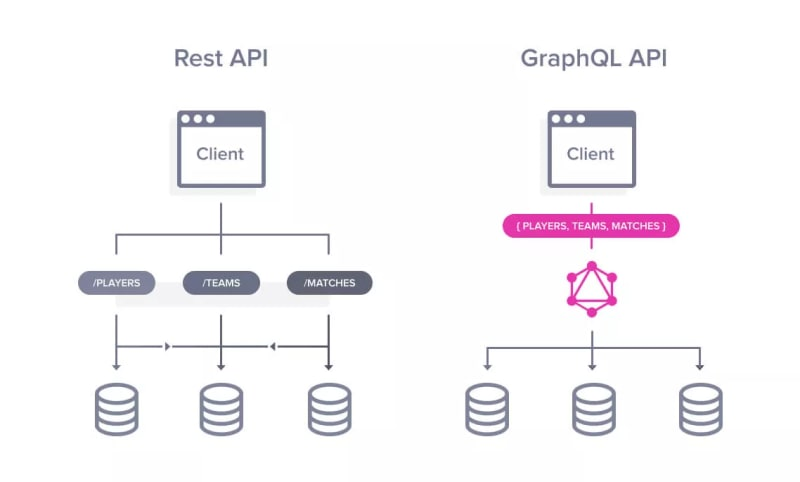
\includegraphics[width=0.8\textwidth]{Figures/graphql.jpg}
    \caption{GraphQL vs. REST Architecture}
    \label{fig:graphqlvsrestarchitecture}
\end{figure}
\begin{multicols}{2} % (json-rpc, xml-rpc, grpc) Webhooks API, Socket API Database API, Third-party API, Apache Thrift API, MsgPack API, SSE API, 
    \textbf{RPC API} : \acrshort{rpc} is a protocol return \acrshort{xml} or \acrshort{json} response. This protocol
    calls a method rather than a data resource, and remains one of the oldest and most stable protocols for
    \acrshort{api}s. While \acrshort{rest}ful \acrshort{api} returns a document, the response from a \acrshort{rpc}
    server is a confirmation that the function was triggered, or an error indicating  why it failed to run.

    \acrshort{rpc} is much faster than \acrshort{rest}, but the specifics depend on implementation. Unlike
    \acrshort{rest} or \acrshort{soap}, the message format varies. \acrshort{rpc} is tailored toward a client-server
    architecture and generally over a network.

    Components of a \acrshort{rpc} system:
    \begin{itemize}[label=$\star$]
        \item Client: the requesting device.
        \item Client stub: how the client will pack/unpack its materials.
        \item \acrshort{rpc} runtime: the messaging system (a courier between the client and server).
        \item Server stub: how the server will pack/unpack its materials.
        \item Server: the supplying device.
    \end{itemize}

    The popular frameworks of \acrshort{rpc}s are Apache Thrift, \acrshort{grpc}, and \acrshort{json}-\acrshort{rpc},
    and \acrshort{xml}-\acrshort{rpc}.

    \textit{gRPC}: developed by Google and released to public in 2015 to use, \acrshort{grpc} is an open-source
    \acrshort{rpc} architecture that can operate in numerous environments.

    The \acrshort{grpc} transport layer primarily relies on \acrshort{http}. The ability for developers to specify
    custom functions that allow for flexible inter-service communication is a significant feature of \acrshort{grpc}.
    This \acrshort{api} protocol also offers extra features such as timeouts, authentication, and flow control.

    In the \acrshort{grpc} protocol, data is transmitted in protocol buffers, a platform and language-agnostic mechanism
    that allows for data to be structured intuitively. This mechanism defines the service and then the data structures
    that the service will use. Compiling is taken care by protoc, the protocol buffer compiler.

    The output of this process is a comprehensive class containing the user's defined data types and basic set of methods
    in the chosen development language. Users can implement in-depth \acrshort{api} operations using this class.
\end{multicols}

\begin{lstlisting}[caption=gRPC Service For a Calculator In a Protobuf File]
      syntax = "proto3";

      package calculator;

      service Calculator {
            rpc Add(AddRequest) returns (AddResponse);
            rpc Subtract(SubtractRequest) returns (SubtractResponse);
      }

      message AddRequest {
            int32 a = 1;
            int32 b = 2;
      }

      message AddResponse {
            int32 result = 1;
      }

      message SubtractRequest {
            int32 a = 1;
            int32 b = 2;
      }

      message SubtractResponse {
            int32 result = 1;
      }
\end{lstlisting}

\begin{multicols}{2}
    \textit{Apache Thrift}: developed by Facebook, Thrift itself is a lightweight, language-agnostic software stack.
    This \acrshort{api} protocol supports \acrshort{http} transmission, along with binary transport formats. Thrift
    is capable of clean abstraction and implementations for data serialization and transport and application-level
    processing. Its primary objective is point-to-point \acrshort{rpc} implementation.

    Apache can support 28 programming languages, allowing programs written in any of these languages to communicate
    with each other and request remote services using \acrshort{api}s.
    \textbf{WebSocket}:
\end{multicols}

\begin{lstlisting}[language=JavaScript, caption=WebSocket's Example]
      // Client-side code
      const socket = new WebSocket('wss://example.com/socket'); // Replace with actual server's websocket URL
      
      // Event handler for when the connection is established
      socket.addEventListener("open", (event) => {
            console.log('Connected to the server');
            // Send data to the server
            socket.send('Hello, server!');
      });

      // Event handler for incoming messages from the server
      socket.addEventListener("message", (event) => {
            console.log(`Message from server: ${event.data}`);	
      });

      // Event handler for when the connection is closed
      socket.addEventListener("close", (event) => {
            console.log('Connection to the server closed');
      });

      // Event hander for handling errors
      socket.addEventListener("error", (event) => {
            console.error(`An error occurred: ${event.message}`);
      });
\end{lstlisting}

\begin{multicols}{2}
    \textbf{Socket}: is a software abstraction that allows programs running on different devices to
    communicate with each other over a network. It provides a standard interface for network
    communication, enabling data to be sent and received between applications running on separate
    computers. Sockets are commonly used in networking applications to establish connections and
    exchange data.
\end{multicols}

\begin{lstlisting}[language=Python, caption=TCP Server Example Using Sockets in Python]
      import socket

      # Create a TCP/IP socket
      server_socket = socket.socket(socket.AF_INET, socket.SOCK_STREAM)

      # Bind the socket to the address and port
      server_address = ('localhost', 8080)
      server_socket.bind(server_address)

      # Listen for incoming connections (max 5 clients in the queue)
      server_socket.listen(5)

      print('Server is listening on port 8080 for incoming connections....')

      while True:
            # Wait for a connection
            client_socket, client_address = server_socket.accept()

            try:
                  # Receive data from the client
                  data = client_socket.recv(1024)
                  print(f"Received data from {client_address}: {data.decode('utf-8')}")

                  # Send a response back to the client
                  response = 'Hello, client!'
                  client_socket.sendall(response.encode('utf-8'))

            finally:
                  # Clean up and close the connection
                  client_socket.close()
\end{lstlisting}

\begin{multicols}{2}
    \textbf{MsgPack}: is an open standard for compact binary data serialization, ideal for efficient data transfer.
    \acrshort{msgpack} supports a variety of data types, including integers, floating-point numbers, strings,
    arrays, maps (key-value pairs), and more. It is designed to be platform-agnostic, meaning that the data can be
    serialized in one programming language and deserialize it in another without compactibility issues.
\end{multicols}

\begin{lstlisting}[language=Python, caption=MsgPack Serialization and Deserialization in Python]
      import msgpack

      # Creating a Python dictionary to represent some data
      data = {
            'name': 'John Doe',
            'age': 30,
            'is_student': False,
            'hobbies': ['Reading', 'Gaming', 'Traveling'],
            'address': {
                  'street': 'Sesame Main Street',
                  'city': 'New York',
                  'zip': '10001'
            }
            "scores": [90, 85, 95, 100, 95, 88, 72]
      }

      # Serialize the data to a MsgPack binary format
      packed_data = msgpack.packb(data)

      # Deserialize the MsgPack binary data back to a Python object
      unpacked_data = msgpack.unpackb(packed_data)

      # Print the original data and the deserialized data
      print("Original data:", data)
      print("Unpacked data:", unpacked_data)
\end{lstlisting}


\subsection{What is API Monitoring?}
\acrshort{api} monitoring is the process of gathering, visualizing, tracking, analyzing, and alerting on the
performance, availability, and the \acrshort{api} telemetry data to ensure that \acrshort{api} requests are
handled as expected.
\subsection{How Does API Monitoring Work?}
\acrshort{api} monitoring automatically checks \acrshort{api} performance and availability at regular intervals,
to ensure that the \acrshort{api} runs appropriately. This can be done in a few different ways, depending on the
type of the \acrshort{api} being monitored~\ref{chap:typesofapis}.

For example, let's take Postman, a popular free \acrshort{api} monitoring tools that allows developers to easily
monitor, analyze, and debug their \acrshort{api}s. In this example, the system might look for common errors, such
as 500-level responses or timeouts, when making requests to the \acrshort{api}. It also checks for latency issues
or sudden spikes in traffic that could indicate potential system problems. In addition, this monitoring system can
be configured to track specific metrics such as total requests, response times, and other \acrshort{kpi}s over time.
This will then provide real-time insights into \acrshort{api} performance and offers a range of features such as
automated alerts, detailed analytics, and comprehensive reporting capabilities. Features that an \acrshort{api}
monitoring might have are listed in the following (\cite{postmanapimonitoring}):
\begin{itemize}
    \item \textbf{Endpoint Surveillance}: it begins by closely tracking the various endpoints of an \acrshort{api}
          system. These endpoints represent specific functionalities or resources that the \acrshort{api} provides.
    \item \textbf{Request-Response Analysis}: monitoring tools can simulate \acrshort{api} requests by sending
          predefined inputs and parameters to specific endpoints, then analyzing the responses for relevant factors
          such as response time or data accuracy.
    \item \textbf{Performance Metrics Measurement}: \acrshort{kpi}s, such as response time, latency, and error rates,
          are measured and tracked over time. This metrics offers insights into the overall health and efficiency of
          an \acrshort{api}.
    \item \textbf{Error Detection and Logging}: actively identifying and log any errors or anomalies in \acrshort{api}
          resources with an \acrshort{api} monitoring program. This includes capturing \acrshort{http} error codes,
          unexpected data/file formats, and alerting of any deviations from expected behaviour.
    \item \textbf{Security Checks}: \acrshort{api} monitoring assess \acrshort{api} transactions for unauthorized
          access attempts, potential vulnerabilities, and adherence to security protocols.
    \item \textbf{Alerting and Notification System}: automated alerting systems can be configured with high levels of
          customization to notify relevant stakeholders when specific \acrshort{api} performance thresholds are breached
          or exceeded or when abnormal behaviour is detected.
    \item \textbf{Usage Analysis Gathering}: collect usage analytics for insights into how a given \acrshort{api} is
          being used. This data helps software organizations plan for scalability, optimize resource allocation, and
          understand user behaviour.
    \item \textbf{Logging for Auditing}: detailed logs of \acrshort{api} interactions are maintained for auditing
          purposes. These \acrshort{api} logs are valuable resources for post-incident analysis and tracking historical
          performance and behavioural trends.
    \item \textbf{Continuous Monitoring}: the tool is a constantly ongoing, real-time process that ensures that
          issues of any scope are identified and addressed promptly.
\end{itemize}
With those functionalities in mind, \acrshort{api} monitoring tools can then automatically check \acrshort{api}
performance and availability at specified intervals of time to ensure that the monitored \acrshort{api}s run
appropriately. The specific timing of those intervals is unique to each \acrshort{api} product.